\section{GrassRoute and Theoretical Guarantees}
Figure~\ref{fig:method} shows one optimizer step; Table~\ref{tab:method-update}
gives the complete updates.
\begin{figure*}[t]
\centering
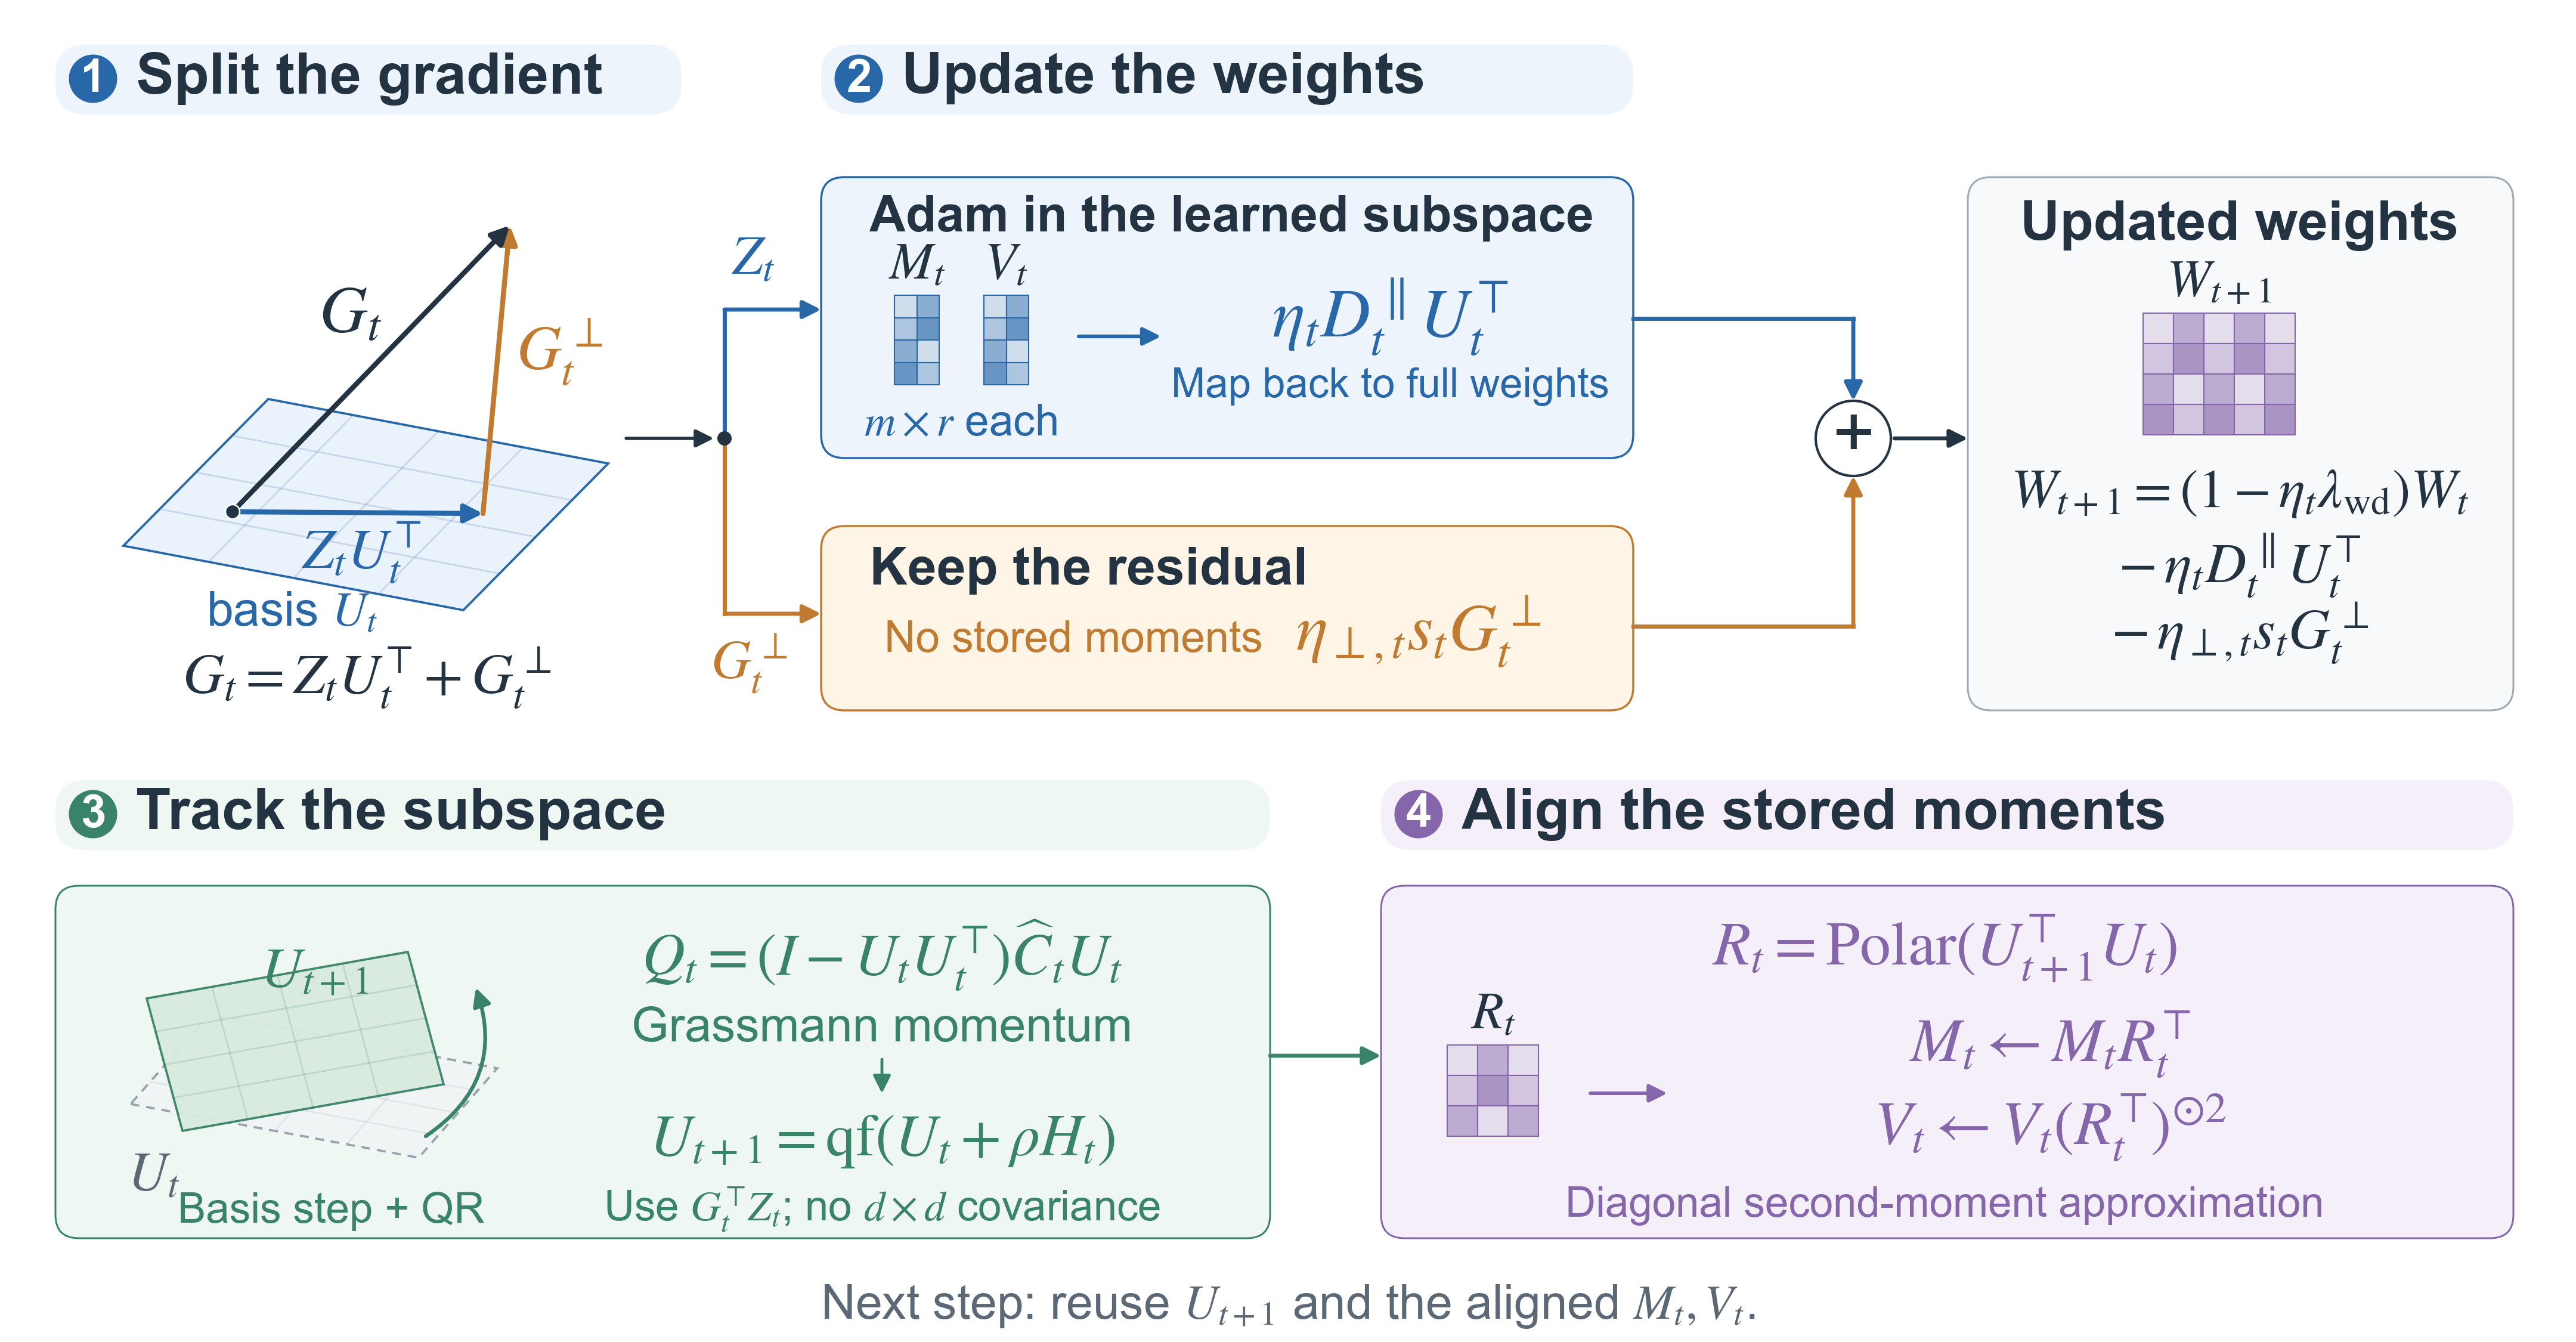
\includegraphics[width=\linewidth]{figures/fig_method_update_detailed.png}
\caption{One GrassRoute step. Adam acts in a learned rank-$r$ subspace,
while a stateless residual branch preserves the remaining gradient directions.
A Grassmann momentum step and QR retraction update the basis. Procrustes
alignment carries the stored moments to the new coordinates; the second-moment
rule approximates the covariance by its diagonal. The geometry is schematic.}
\label{fig:method}
\end{figure*}
% WWW table style: three rules, bold headers, reference green highlight.
\begin{table}[t]
\centering\footnotesize
\caption{\textbf{One GrassRoute iteration.} The parameter branch preserves the full orthogonal residual; the routing branch changes the basis and aligns stored coordinates. Second-moment transport is a diagonal approximation. Elementwise operations use $\oslash$ and $\odot$.}
\label{tab:method-update}
\setlength{\tabcolsep}{5pt}
\reviewfit{\begin{tabular}{@{}p{.17\linewidth}p{.62\linewidth}p{.14\linewidth}@{}}
\toprule {\bfseries Stage} & {\bfseries Update} & {\bfseries Stored state}\\
\midrule
Project gradient  &  $Z_t=G_tU_t,\quad G_t^\perp=G_t-Z_tU_t^\top$  &  $U_t\in\mathbb R^{d\times r}$\\
Adaptive moments  &  $M_t=\beta_1M_{t-1}+(1-\beta_1)Z_t,\quad V_t=\beta_2V_{t-1}+(1-\beta_2)Z_t^{\odot2}$  &  $2mr$ entries\\
Bias correction  &  $\widehat M_t=M_t/(1-\beta_1^t),\quad\widehat V_t=V_t/(1-\beta_2^t)$  &  Moment ages\\
Adaptive branch  &  $D_t^\parallel=\widehat M_t\oslash(\sqrt{\widehat V_t}+\varepsilon)$  &  No $m\times d$ moments\\
Residual branch  &  $s_t=\operatorname{clip}(\|G_t\|_F/(\|G_t^\perp\|_F+\varepsilon_r);s_{\min},s_{\max})$  &  Stateless\\
\rowcolor{oursbg}
Parameter update  &  $W_{t+1}=(1-\eta_t\lambda_{\rm wd})W_t-\eta_tD_t^\parallel U_t^\top-\eta_{\perp,t}s_tG_t^\perp$  &  Full $W_t$\\
\midrule
Horizontal direction  &  $Q_t=(I-U_tU_t^\top)G_t^\top Z_t/(\|G_t\|_F^2+\varepsilon_c)$  &  No full covariance\\
Transported momentum  &  $H_t=\mu_H\Pi_{U_t}H_{t-1}+(1-\mu_H)Q_t$  &  $dr$ entries\\
\rowcolor{oursbg}
Grassmann update  &  $U_{t+1}=\operatorname{qf}(U_t+\rho_tH_t)$  &  $dr$ basis entries\\
Coordinate alignment  &  $R_t=\operatorname{Polar}(U_{t+1}^\top U_t),\quad M_t\leftarrow M_tR_t^\top$  &  $r\times r$ rotation\\
Diagonal transport  &  $V_t\leftarrow V_t(R_t^\top)^{\odot2}$  &  Same moment age\\
\bottomrule
\end{tabular}}
\end{table}

The routed branch maintains Adam moments of $Z_t$, producing $D_t^\parallel$. The residual branch uses
\begin{align}
s_t&=\operatorname{clip}\left(\frac{\|G_t\|_F}{\|G_t^\perp\|_F+\varepsilon_r};s_{\min},s_{\max}\right),\\
W_{t+1}&=(1-\eta_t\lambda_{\rm wd})W_t-\eta_tD_t^\parallel U_t^\top\notag\\
&\quad-\eta_{\perp,t}s_tG_t^\perp.
\end{align}
For $\widehat C_t=G_t^\top G_t/(\|G_t\|_F^2+\varepsilon_c)$, the tracker ascends along $Q_t=(I-P_t)\widehat C_tU_t$. Computing $G_t^\top(G_tU_t)$ avoids constructing a $d\times d$ covariance.



The positive sign follows the ascent direction of captured energy. Residual
norm matching uses the raw gradient norm, so its effective step scale can
differ substantially from Adam's (Proposition~\ref{prop:branch-scale}).
Moment alignment retains the diagonal of a rotated diagonal covariance and
discards unavailable cross-correlations. Adam therefore remains coordinate
dependent. Lemma~\ref{lem:moments} compares this rule with the archived
amplitude-rotation and hard-reset variants, which we report separately.
Lemma~\ref{lem:qr} bounds the QR--exponential discrepancy on the Grassmann
quotient by a cubic term in the tangent step.

\paragraph{Landscape and tracking.}
Theorem~\ref{thm:landscape} gives, for $\theta_{\max}\le R_0<\pi/2$,
\begin{equation}
\|\operatorname{grad}\Phi_t(U)\|_F^2\ge2\Delta_t\cos^2R_0\{\Phi_t(U)-\Phi_t(U_t^\star)\}.
\end{equation}
Principal-coordinate Rayleigh quotients yield this bound. A CS/Poincar\'e
reduction gives the sharp QR pullback constant
$L_R=\lambda_1(C_t)-\lambda_d(C_t)$ without an ambient-dimension factor.
Neither quadratic growth nor PL implies geodesic strong convexity over this
whole region. The tracking recursion in Theorem~\ref{thm:tracking} separates
sampling noise, covariance drift, and momentum bias. Its steady-state terms
include $\rho\sigma^2/\mu$, $B^2/\mu$, and
$v^2/(\rho^2\mu^2\Delta_0)$, where $\mu=\Delta_0\cos^2R_0$ and $v$ bounds
covariance change. Thus smaller routing steps reduce sampling noise but
increase sensitivity to target drift.

\paragraph{Convergence.}
Theorem~\ref{thm:convergence} bounds nonconvex stationarity while retaining
the error from adaptive directions. Under Assumption~\ref{ass:actual-adam},
including bounded gradients and conditionally radial unimodal noise,
Theorem~\ref{thm:actual-adam} controls this error for
the transported moments and current-batch denominator. A virtual iterate
cancels first-moment history; averaging before applying Cauchy--Schwarz and
Minkowski gives a scalar quadratic-root bound. The induced direction error
has a mean-square upper bound proportional to $c_t=(1-\beta_2)/(1-\beta_2^t)$
(Lemma~\ref{lem:predictable-denominator}). With
$\eta,\rho\asymp T^{-1/2}$ and $\beta_2=1-1/T$, the stationarity rate is
$O(T^{-1/2})+O((\log T)/T)+O(\varepsilon_r^2)$. A positive residual floor
removes the last term under the same noise assumptions; these assumptions
are not verified for the benchmark runs. Corollary~\ref{cor:deterministic-adam}
treats deterministic bounded gains. With a positive residual-gain lower bound,
rank truncation need not impose a fixed error floor
(Proposition~\ref{prop:no-tail-floor}).

\paragraph{Generalization.}
Theorem~\ref{thm:generalization} couples the full optimizer state on
neighboring i.i.d. data sets. Propositions~\ref{prop:explicit-state-constants}
and~\ref{prop:spectral-feedback} give a five-state sensitivity matrix and
conditions controlling its feedback. A separate PAC-Bayes analysis retains
the exact Gaussian orientation cost and the Seeger--Maurer binary-KL inverse
(Theorems~\ref{thm:angle-KL} and~\ref{thm:Seeger-Maurer}). Davis--Kahan and
McDiarmid--Tropp bounds connect this cost to tracking error; the certificate
based on observed angles needs no eigengap (Theorem~\ref{thm:tracking-PAC}).
For a Gaussian head on fixed features, one-dimensional conditioning gives
the exact empirical Gibbs error (Proposition~\ref{prop:pb-margin}).
Appendix~\ref{app:validation-selection} separately accounts for finite
validation selection. These conditional results are not evaluated numerical
certificates for the deep networks in our experiments.

\paragraph{Compatibility and sharper local results.}
With spherical gradient noise and a fixed positive covariance offset,
Theorem~\ref{thm:gap-collapse} gives
$\Delta_{r,t}\le2\|\nabla f(W_t)\|^2/\varepsilon_c$.
A uniform positive-gap tracking guarantee therefore cannot extend unchanged
to the stationarity limit. Theorem~\ref{thm:basin-certificate} instead
certifies a finite tracking window. Theorems~\ref{thm:modal-tracking-covariance}
and~\ref{thm:rankone-QR-Lyapunov} give exact additive-oracle modal error and
an invariant neighborhood for the deterministic rank-one tracker.
Theorem~\ref{thm:neutral-routing-stability} allows noncontractive routing
when its feedback is summable. For generalization, a Haar mixture prior
accounts for learned orientation through an explicit orbital partition
function; its large-concentration cost has leading term
$\tfrac12r(d-r)\log c$. Table~\ref{tab:proof-sharpness} lists the equality
cases and the terms that remain conservative.
